\documentclass[]{article}
\usepackage[left=1in,top=1in,right=1in,bottom=1in]{geometry}


%%%% more monte %%%%
% thispagestyle{empty}
% https://stackoverflow.com/questions/2166557/how-to-hide-the-page-number-in-latex-on-first-page-of-a-chapter
\usepackage{color}
% \usepackage[table]{xcolor} % are they using color?

% \definecolor{WSU.crimson}{HTML}{981e32}
% \definecolor{WSU.gray}{HTML}{5e6a71}

% \definecolor{shadecolor}{RGB}{248,248,248}
\definecolor{WSU.crimson}{RGB}{152,30,50} % use http://colors.mshaffer.com to convert from 981e32
\definecolor{WSU.gray}{RGB}{94,106,113}

%%%%%%%%%%%%%%%%%%%%%%%%%%%%

\newcommand*{\authorfont}{\fontfamily{phv}\selectfont}
\usepackage{lmodern}


  \usepackage[T1]{fontenc}
  \usepackage[utf8]{inputenc}




\usepackage{abstract}
\renewcommand{\abstractname}{}    % clear the title
\renewcommand{\absnamepos}{empty} % originally center

\renewenvironment{abstract}
 {{%
    \setlength{\leftmargin}{0mm}
    \setlength{\rightmargin}{\leftmargin}%
  }%
  \relax}
 {\endlist}

\makeatletter
\def\@maketitle{%
  \pagestyle{empty}
  \newpage
%  \null
%  \vskip 2em%
%  \begin{center}%
  \let \footnote \thanks
    {\fontsize{18}{20}\selectfont\raggedright  \setlength{\parindent}{0pt} \@title \par}%
}
%\fi
\makeatother






\usepackage{color}
\usepackage{fancyvrb}
\newcommand{\VerbBar}{|}
\newcommand{\VERB}{\Verb[commandchars=\\\{\}]}
\DefineVerbatimEnvironment{Highlighting}{Verbatim}{commandchars=\\\{\}}
% Add ',fontsize=\small' for more characters per line
\usepackage{framed}
\definecolor{shadecolor}{RGB}{248,248,248}
\newenvironment{Shaded}{\begin{snugshade}}{\end{snugshade}}
\newcommand{\AlertTok}[1]{\textcolor[rgb]{0.94,0.16,0.16}{#1}}
\newcommand{\AnnotationTok}[1]{\textcolor[rgb]{0.56,0.35,0.01}{\textbf{\textit{#1}}}}
\newcommand{\AttributeTok}[1]{\textcolor[rgb]{0.77,0.63,0.00}{#1}}
\newcommand{\BaseNTok}[1]{\textcolor[rgb]{0.00,0.00,0.81}{#1}}
\newcommand{\BuiltInTok}[1]{#1}
\newcommand{\CharTok}[1]{\textcolor[rgb]{0.31,0.60,0.02}{#1}}
\newcommand{\CommentTok}[1]{\textcolor[rgb]{0.56,0.35,0.01}{\textit{#1}}}
\newcommand{\CommentVarTok}[1]{\textcolor[rgb]{0.56,0.35,0.01}{\textbf{\textit{#1}}}}
\newcommand{\ConstantTok}[1]{\textcolor[rgb]{0.00,0.00,0.00}{#1}}
\newcommand{\ControlFlowTok}[1]{\textcolor[rgb]{0.13,0.29,0.53}{\textbf{#1}}}
\newcommand{\DataTypeTok}[1]{\textcolor[rgb]{0.13,0.29,0.53}{#1}}
\newcommand{\DecValTok}[1]{\textcolor[rgb]{0.00,0.00,0.81}{#1}}
\newcommand{\DocumentationTok}[1]{\textcolor[rgb]{0.56,0.35,0.01}{\textbf{\textit{#1}}}}
\newcommand{\ErrorTok}[1]{\textcolor[rgb]{0.64,0.00,0.00}{\textbf{#1}}}
\newcommand{\ExtensionTok}[1]{#1}
\newcommand{\FloatTok}[1]{\textcolor[rgb]{0.00,0.00,0.81}{#1}}
\newcommand{\FunctionTok}[1]{\textcolor[rgb]{0.00,0.00,0.00}{#1}}
\newcommand{\ImportTok}[1]{#1}
\newcommand{\InformationTok}[1]{\textcolor[rgb]{0.56,0.35,0.01}{\textbf{\textit{#1}}}}
\newcommand{\KeywordTok}[1]{\textcolor[rgb]{0.13,0.29,0.53}{\textbf{#1}}}
\newcommand{\NormalTok}[1]{#1}
\newcommand{\OperatorTok}[1]{\textcolor[rgb]{0.81,0.36,0.00}{\textbf{#1}}}
\newcommand{\OtherTok}[1]{\textcolor[rgb]{0.56,0.35,0.01}{#1}}
\newcommand{\PreprocessorTok}[1]{\textcolor[rgb]{0.56,0.35,0.01}{\textit{#1}}}
\newcommand{\RegionMarkerTok}[1]{#1}
\newcommand{\SpecialCharTok}[1]{\textcolor[rgb]{0.00,0.00,0.00}{#1}}
\newcommand{\SpecialStringTok}[1]{\textcolor[rgb]{0.31,0.60,0.02}{#1}}
\newcommand{\StringTok}[1]{\textcolor[rgb]{0.31,0.60,0.02}{#1}}
\newcommand{\VariableTok}[1]{\textcolor[rgb]{0.00,0.00,0.00}{#1}}
\newcommand{\VerbatimStringTok}[1]{\textcolor[rgb]{0.31,0.60,0.02}{#1}}
\newcommand{\WarningTok}[1]{\textcolor[rgb]{0.56,0.35,0.01}{\textbf{\textit{#1}}}}



\title{\textbf{\textcolor{WSU.crimson}{The Influence of Biological Sex on Human Body Part Ratios}} \newline \textbf{\textcolor{WSU.gray}{How these Ratios Compare Between the Sexes}}  }

%  

% \author{ \Large true \hfill \normalsize \emph{} }
\author{\Large Kevin A. Black -
\href{mailto:kevin.black@wsu.edu}{\nolinkurl{kevin.black@wsu.edu}}\vspace{0.05in} \newline\normalsize\emph{Washington State University Vancouver}  }


\date{November 01, 2020}
\setcounter{secnumdepth}{3}

\usepackage{titlesec}
% See the link above: KOMA classes are not compatible with titlesec any more. Sorry.
% https://github.com/jbezos/titlesec/issues/11
\titleformat*{\section}{\bfseries}
\titleformat*{\subsection}{\bfseries\itshape}
\titleformat*{\subsubsection}{\itshape}
\titleformat*{\paragraph}{\itshape}
\titleformat*{\subparagraph}{\itshape}

% https://code.usgs.gov/usgs/norock/irvine_k/ip-092225/


%\titleformat*{\section}{\normalsize\bfseries}
%\titleformat*{\subsection}{\normalsize\itshape}
%\titleformat*{\subsubsection}{\normalsize\itshape}
%\titleformat*{\paragraph}{\normalsize\itshape}
%\titleformat*{\subparagraph}{\normalsize\itshape}

% https://tex.stackexchange.com/questions/233866/one-column-multicol-environment#233904
\usepackage{environ}
\NewEnviron{auxmulticols}[1]{%
  \ifnum#1<2\relax% Fewer than 2 columns
    %\vspace{-\baselineskip}% Possible vertical correction
    \BODY
  \else% More than 1 column
    \begin{multicols}{#1}
      \BODY
    \end{multicols}%
  \fi
}





\usepackage{natbib}
\setcitestyle{aysep={}} %% no year, comma just year
% \usepackage[numbers]{natbib}
\bibliographystyle{./../biblio/ormsv080.bst}



\usepackage[strings]{underscore} % protect underscores in most circumstances




\newtheorem{hypothesis}{Hypothesis}
\usepackage{setspace}


%%%%%%%%%%%%%%%%%%%%%%%%%%%%%%%%%%%%%%%%%%%%%%%%%%%%%
%%% MONTE ADDS %%%

\usepackage{fancyhdr} % fancy header 
\usepackage{lastpage} % last page 

\usepackage{multicol}


\usepackage{etoolbox}
\AtBeginEnvironment{quote}{\singlespacing\small}
% https://tex.stackexchange.com/questions/325695/how-to-style-blockquote


\usepackage{soul}			%% allows strike-through
\usepackage{url}			%% fixes underscores in urls
\usepackage{csquotes}		%% allows \textquote in references
\usepackage{rotating}		%% allows table and box rotation
\usepackage{caption}		%% customize caption information
\usepackage{booktabs}		%% enhance table/tabular environment
\usepackage{tabularx}		%% width attributes updates tabular
\usepackage{enumerate}		%% special item environment
\usepackage{enumitem}		%% special item environment

\usepackage{lineno}		%% allows linenumbers for editing using \linenumbers
\usepackage{hanging}


\usepackage{mathtools}  	%% also loads amsmath
\usepackage{bm}		%% bold-math
\usepackage{scalerel}	%% scale one element (make one beta bigger font)

\newcommand{\gFrac}[2]{ \genfrac{}{}{0pt}{1}{{#1}}{#2} }

\newcommand{\betaSH}[3]{  \gFrac{\text{\tiny #1}}{{\text{\tiny #2}}}\hat{\beta}_{\text{#3}}   }
\newcommand{\betaSB}[3]{              ^{\text{#1}} _{\text{#2}} \bm{\beta} _{\text{#3}}                   }  %% bold
\newcommand{\bigEQ}{  \scaleobj{1.5}{{\ }= } }
\newcommand{\bigP}[1]{  \scaleobj{1.5}{#1 } }





\usepackage{endnotes}  % he already does this ...
\renewcommand{\enotesize}{\normalsize}
% https://tex.stackexchange.com/questions/99984/endnotes-do-not-be-superscript-and-add-a-space
\renewcommand\makeenmark{\textsuperscript{[\theenmark]}} % in brackets %
% https://tex.stackexchange.com/questions/31574/how-to-control-the-indent-in-endnotes
\patchcmd{\enoteformat}{1.8em}{0pt}{}{}

\patchcmd{\theendnotes}
  {\makeatletter}
  {\makeatletter\renewcommand\makeenmark{\textbf{[\theenmark]} }}
  {}{}



% https://tex.stackexchange.com/questions/141906/configuring-footnote-position-and-spacing

\addtolength{\footnotesep}{5mm} % change to 1mm

\renewcommand{\thefootnote}{\textbf{\arabic{footnote}}}
\let\footnote=\endnote
%\renewcommand*{\theendnote}{\alph{endnote}}
%\renewcommand{\theendnote}{\textbf{\arabic{endnote}}}


\renewcommand*{\notesname}{ENDNOTES}

\makeatletter
\def\enoteheading{\section*{\notesname
  \@mkboth{\MakeUppercase{\notesname}}{\MakeUppercase{\notesname}}}%
  \mbox{}\par\vskip-2.3\baselineskip\noindent\rule{.5\textwidth}{0.4pt}\par\vskip\baselineskip}
\makeatother


\renewcommand*{\contentsname}{TABLE OF CONTENTS}

\renewcommand*{\refname}{REFERENCES}


%\usepackage{subfigure}
\usepackage{subcaption}

\captionsetup{labelfont=bf}  % Make Table / Figure bold

%%% you could add elements here ... monte says .... %%%
%\usepackage{mypackageForCapitalH}


%%%%%%%%%%%%%%%%%%%%%%%%%%%%%%%%%%%%%%%%%%%%%%%%%%%%%

% set default figure placement to htbp
\makeatletter
\def\fps@figure{htbp}
\makeatother

\usepackage{hyperref}

% move the hyperref stuff down here, after header-includes, to allow for - \usepackage{hyperref}

\makeatletter
\@ifpackageloaded{hyperref}{}{%
\ifxetex
  \PassOptionsToPackage{hyphens}{url}\usepackage[setpagesize=false, % page size defined by xetex
              unicode=false, % unicode breaks when used with xetex
              xetex]{hyperref}
\else
  \PassOptionsToPackage{hyphens}{url}\usepackage[draft,unicode=true]{hyperref}
\fi
}

\@ifpackageloaded{color}{
    \PassOptionsToPackage{usenames,dvipsnames}{color}
}{%
    \usepackage[usenames,dvipsnames]{color}
}
\makeatother
\hypersetup{breaklinks=true,
            bookmarks=true,
            pdfauthor={Kevin A. Black -
\href{mailto:kevin.black@wsu.edu}{\nolinkurl{kevin.black@wsu.edu}} (Washington State University Vancouver)},
             pdfkeywords = {multiple comparisons to control; multivariate chi-square distribution;
nonlinear growth curves; Richard's curve; simulated critical points},  
            pdftitle={The Influence of Biological Sex on Human Body Part Ratios: How these Ratios Compare Between the Sexes},
            colorlinks=true,
            citecolor=blue,
            urlcolor=blue,
            linkcolor=magenta,
            pdfborder={0 0 0}}
\urlstyle{same}  % don't use monospace font for urls

% Add an option for endnotes. -----

%
% add tightlist ----------
\providecommand{\tightlist}{%
\setlength{\itemsep}{0pt}\setlength{\parskip}{0pt}}

% add some other packages ----------

% \usepackage{multicol}
% This should regulate where figures float
% See: https://tex.stackexchange.com/questions/2275/keeping-tables-figures-close-to-where-they-are-mentioned
\usepackage[section]{placeins}



\pagestyle{fancy}   
\lhead{\textcolor{WSU.crimson}{\textbf{ The Influence of Biological Sex on Human Body Part Ratios }}}
\chead{}
\rhead{\textcolor{WSU.gray}{\textbf{  Page\ \thepage\ of\ \protect\pageref{LastPage} }}}
\lfoot{}
\cfoot{}
\rfoot{}


\begin{document}
	
% \pagenumbering{arabic}% resets `page` counter to 1 
%
% \maketitle

{% \usefont{T1}{pnc}{m}{n}
\setlength{\parindent}{0pt}
\thispagestyle{plain}
{\fontsize{18}{20}\selectfont\raggedright 
\maketitle  % title \par  

}

{
   \vskip 13.5pt\relax \normalsize\fontsize{11}{12} 
   
\textbf{\authorfont Kevin A. Black -
\href{mailto:kevin.black@wsu.edu}{\nolinkurl{kevin.black@wsu.edu}}} \hskip 15pt \emph{\small Washington State University Vancouver}   

}

}








\begin{abstract}

    \hbox{\vrule height .2pt width 39.14pc}

    \vskip 8.5pt % \small 

\noindent In this article we compare the \emph{empirical characteristic function}
\citep{Tukey:1977, Becker:1988} to a
\emph{moment-generating-functional form} to compute the proportion of
hypotheses \(m\) that are rejected under the null hypothesis.
\vspace{0.25in}

\noindent Here is a second paragraph of the abstract (if necessary), and
with the pipe notation it doesn't break. Notice it still needs to be
indented. \vspace{0.25in}

\noindent Generally, we write this abstract last. Often it is called the
executive summary. It should succinctly summarize the entire document.
You can include references such as this one to the Appendices section
\ref{sec:appendix} if necessary.


\vskip 8.5pt \noindent \textbf{\underline{Keywords}:} multiple comparisons to control; multivariate chi-square distribution;
nonlinear growth curves; Richard's curve; simulated critical points \par

    




    
    \hbox{\vrule height .2pt width 39.14pc}
    \vskip 5pt 
    \hfill \textbf{\textcolor{WSU.gray}{ November 01, 2020 } }
    \vskip 5pt 
    
\end{abstract}


\vskip -8.5pt



 % removetitleabstract

\noindent  

\section{Introduction}
\label{sec:intro}

As a customary portion of the STAT 419 course at Washington State
University, the students involved were required to take part in a data
collection/manipulation project involving the measurements of various
body parts. Following the data collection, professor Monte Shaffer
compiled all contributions made by the students into a single,
pipe-delimited text file whose explicit content is to remain
confidential and only used for the sake of addressing a variety of
research questions.

\vspace{0.25cm}

After receiving the data set (\(n=428\)) and cleaning up particular
observations using a range of methodologies based on what I had in mind
for how this data will be used, I determined that I would focus on what
kind of influence biological sex has on certain human body part ratios.
To supplement my inquiry of this data, I centered my research questions
around particular measurements of the human body, such as height, arm
span, foot length, distance from elbow to armpit, head height, just to
name a few. Research questions pertaining to this study and supportive R
code can be found below.

\section{How does being male or female influence the ratios between certain body parts?}
\label{sec:rq}

Making particular deductions throughout history regarding body
measurements among males and females is more than likely due to the
distinct patterns one can find when comparing the biological sexes.
Those born as males or females have about as many differing features to
one another than their similar features, both internally and externally.
Internally speaking, men typically have deeper voices, a faster
metabolism, and can easily build muscle mass, whereas women possess a
much more complicated reproductive system, have the ability to
breastfeed, and live longer on average \citep{Wolchover:2011}. What
about externally? How does being male or female influence the ratios
between certain body parts? The latter primary question will be
elaborated through the following sub-questions, focusing on particular
ratios that are likely to yield some insight on the different external
measurements between males and females.

\subsection{How does 'height' compare to 'arm span' between males and females?}
\label{sec:rq2}

Test

\begin{figure}[!ht]
    \begin{center}
        \scalebox{1.00}{    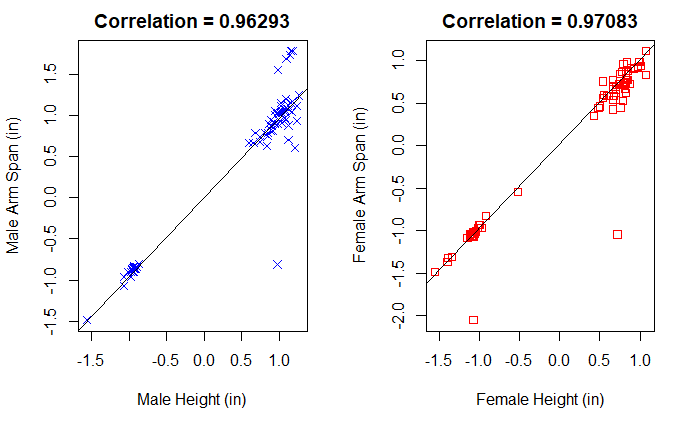
\includegraphics[trim = 0 0 0 0,clip,width=0.85\textwidth]{figures/sq1.png} }
        \caption{Plots and correlation values for males and females regarding height and arm span.}
    \end{center}
    \label{fig:sq1}
\end{figure}

\subsection{How does 'foot length' compare to the length of 'elbow to armpit' between males and females?}
\label{sec:rq3}

\subsection{How many average 'head height' lengths are males and females relative to their respective, average 'height'?}
\label{sec:rq4}

\section{Data Description}
\label{sec:data}

As mentioned in the introduction, the data set utilized throughout this
research paper was supplied through the combined efforts of professor
Monte Shaffer and the students of the STAT 419 class at Washington State
University. Each student was tasked with recording distinct observations
of 37 attributes from 10 different people, ideally with an even mix of
males and females. For each observation (person), there are measurements
of body parts, data collector/respondent identifiers ran through a MD5
hash function, and general information about each respondent. Body part
measurements were recorded using body measuring tape in either inches or
centimeters, but for the sake of consistency throughout the research
paper, all centimeter values were converted to inches and will be
treated as inches from here on.

\vspace{0.25cm}

These observations were recorded in early September 2020 and compiled by
the instructor for our use in late October 2020. Given that these
observations were recorded amid the COVID-19 pandemic, each student was
required to make a simple, yet descriptive handout that would detail how
one would go about recording their own body measurements and the
necessary values to take note of. This would be an ideal situation of
how observations were recorded and sent electronically by each
respondent, but observations could also be taken in person given that
the surveyor and respondent were comfortable being in close proximity of
each other. An example of a two-page handout created by Kevin Black, as
well as further information regarding the attributes of this data set,
can be found in Appendix \ref{sec:appendix-data-handout} and Appendix
\ref{sec:appendix-dataset-ex}, respectively.

\vspace{0.25cm}

On the surface, the purpose for writing this research paper and
collecting the necessary data can simply be attributed to project
requirements for a university course. However, the deeper reasoning
behind why this research paper was composed the first place was to give
students a more thorough understanding of the data analytics process.
More specifically, how to not just work with the data, but how to
understand the data and derive effective questions, how to test for
patterns and conclusions in a statistical, analytic environment, and how
to exercise data provenance practices. This process will be very similar
between all data focused projects in a data analyst's career, so this is
a good starting point for garnering crucial experience.

\section{Key Findings}
\label{sec:findings}

\newpage

\section{APPENDICES}
\label{sec:appendix}

\subsection{Data Provenance}
\label{sec:appendix-data-provenance}

\subsubsection{Utilization of Data Provenance}
\label{sec:appendix-provenance-explained}

While it could be seen as an application mainly used in large-scale data
analytics projects, the multitude of steps to practice data provenance
was also used to handle the vulnerable data used in this research.
Auxiliary files such as the R project files can be found on the
\href{https://github.com/KevnBlack/WSU_STATS419_FALL2020/tree/master/PROJECT-01}{project repository}
through GitHub, while the specific functions used in this report can be
found in the \texttt{functions-project-measure.R}
\href{https://raw.githubusercontent.com/KevnBlack/WSU_STATS419_FALL2020/master/functions/functions-project-measure.R}{file}
or in section \ref{sec:appendix-setup}. The data set itself was not
saved to any location online due to privacy concerns, but it was
organized and saved onto a local hard drive for immediate use.

\vspace{0.25cm}

The collection and general organization process for the data set is
thoroughly described in sections \ref{sec:data} and
\ref{sec:appendix-dataset-ex}. Cleaning for the actual substance of the
data set was performed through the use of the
\texttt{prepareMeasureData()} function, where the data set was
manipulated to more better fit the aims of addressing the particular
research questions for this report. Cleaning this data set involved
multiple steps, such as: omitting rows containing NA values based solely
on the body measurement columns, setting a consistent naming convention
for gender and units, converting all body measurement values to inches,
and scaling the body measurement data. Keeping the research questions in
mind and despite the cleaning of all columns, the only body measurement
fields utilized were \(height\), \(arm.span\), \(foot.length\),
\(elbow.armpit\), and \(head.height\).

\vspace{0.25cm}

Prior to \texttt{prepareMeasureData()}, the data is imported via the
\texttt{read.file()} function where it checks to see if a cleaned
version of the data set already exists, to which that particular file
would take precedence and be used. If no clean version currently exists,
the function goes through the cleaning process and saves the cleaned
data set to the same directory as original data set. For unbiased
samples of the data frame, a seed was set for reproducibility and 200
random observations were drawn without replacement.

\vspace{0.25cm}

The documented R code can be found in section \ref{sec:appendix-setup}.
Key findings and visualizations of summary statistics were discussed
previously throughout sections \ref{sec:rq} through \ref{sec:findings}.
Based on the points made in this section, its clear that data provenance
was kept in mind for making sure there was a traceable history in the
usage of this data set, whether to resolve potential issues or to cut
down on access times.

\newpage

\subsubsection{Data Collection Handout}
\label{sec:appendix-data-handout}

\begin{figure}[!ht]
    \hrule
    \caption{ \textbf{Handout Page 1} }
    \begin{center}
        \scalebox{1.00}{    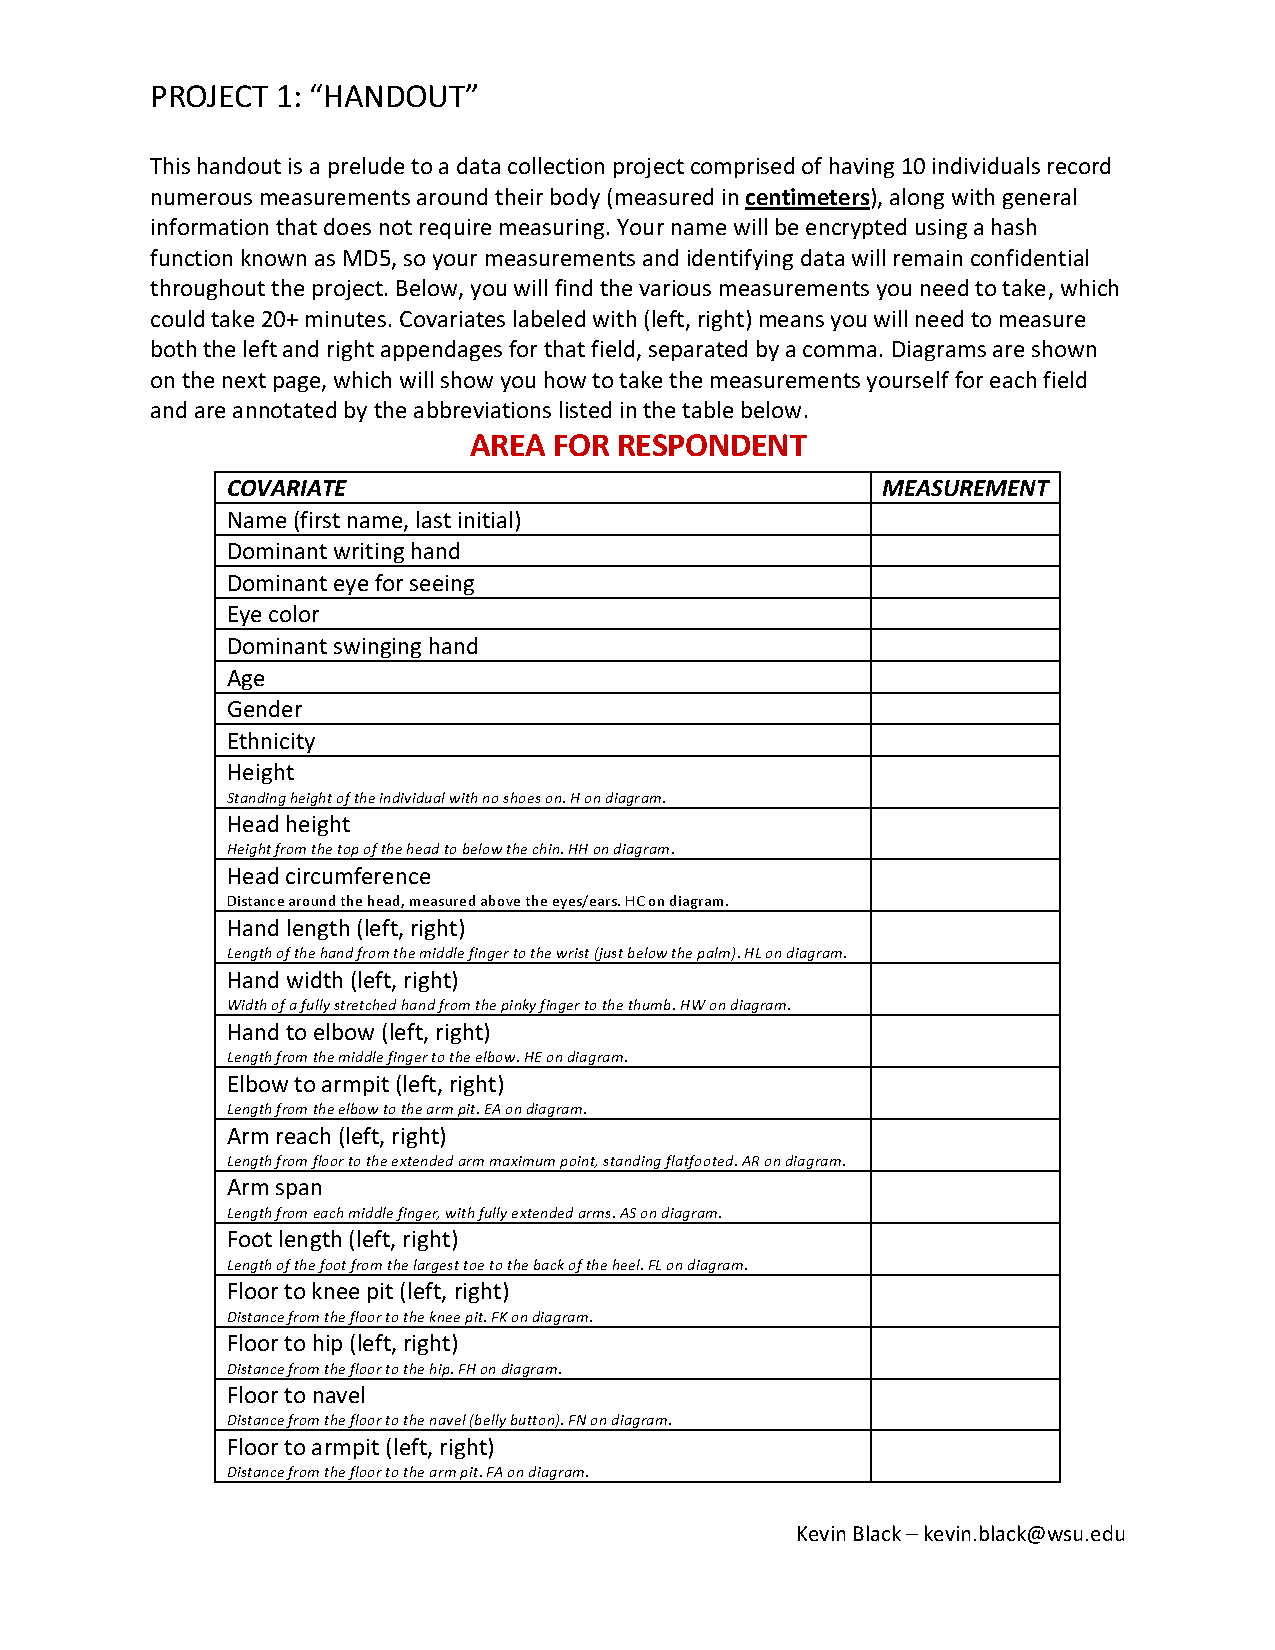
\includegraphics[trim = 0 0 0 0,clip,width=0.85\textwidth]{pdfs/handout1.pdf} }
    \end{center}
    \label{fig:handout-1}
    \hrule
\end{figure}

\newpage

\begin{figure}[!ht]
    \hrule
    \caption{ \textbf{Handout Page 2} }
    \begin{center}
        \scalebox{1.00}{    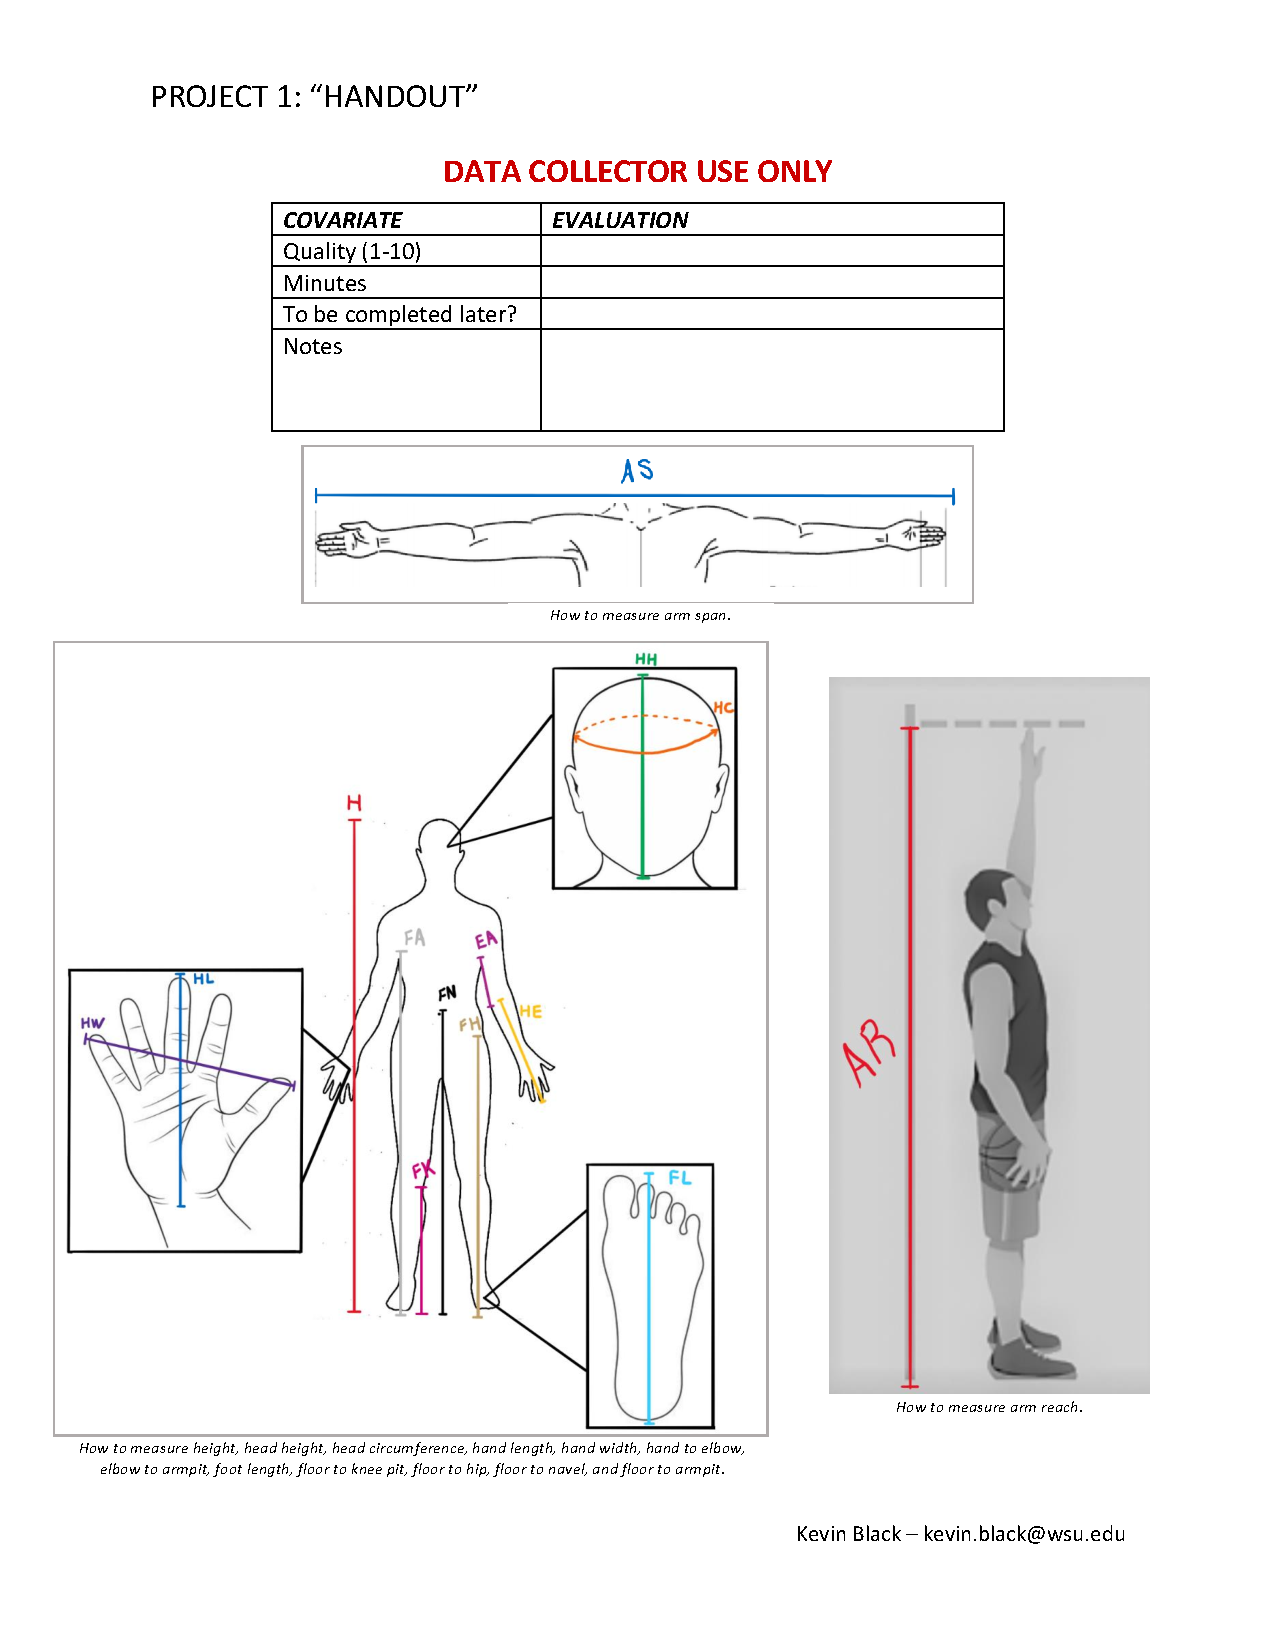
\includegraphics[trim = 0 0 0 0,clip,width=0.85\textwidth]{pdfs/handout2.pdf} }
    \end{center}
    \label{fig:handout-2}
    \hrule
\end{figure}

\newpage

\subsection{Data Set Explained}
\label{sec:appendix-dataset-ex}

In addition to how the data set was described in Section \ref{sec:data},
explanations regarding each attribute can be found below. After the
collaborative effort of all students having their data compiled, the
data set ended up having 428 total observations. However, the data set
was filled with an enormous amount of NA values in the body
measurements, potentially due to the time constraints of some students
or lack of attempt to fill out all fields. As a result, running the
function \texttt{complete.cases()} on the data set during the data
cleaning process returned a data frame containing only 262 observations,
about 61.21\% of the original data set size. \texttt{complete.cases()}
was used over \texttt{na.omit()} because the latter function would omit
all rows containing NA values based on all columns, including the rows
where the non-body measurement attributes had NA values, whereas the
former function would omit NA values only for the specified body
measurement columns.

\begin{figure}[!ht]
    \caption{ \textbf{Description of Each Field} }
    \begin{center}
        \scalebox{1.00}{    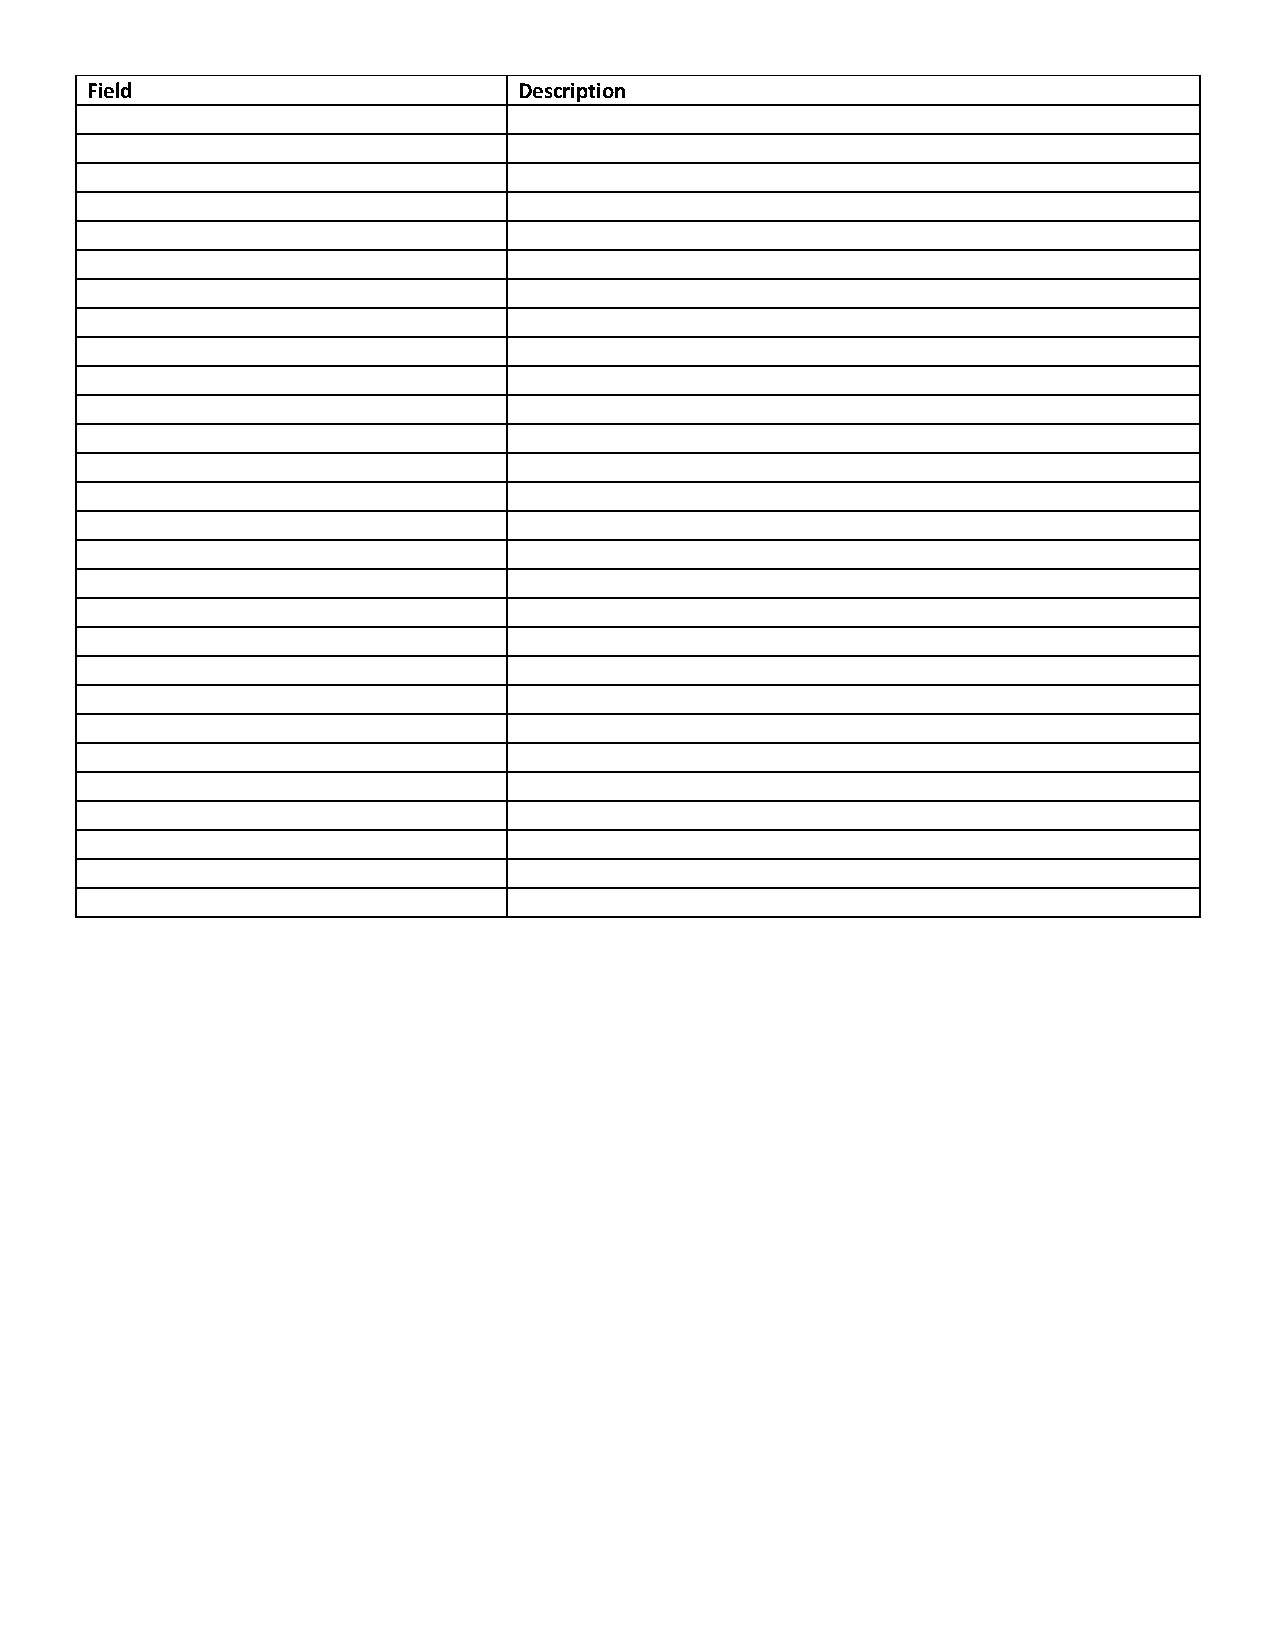
\includegraphics[trim = 0 350 100 35,clip,width=0.85\textwidth]{pdfs/datasets_explained.pdf} }
    \end{center}
    \label{fig:datasets_explained}
\end{figure}

\newpage

\subsection{R Code Used for Research}
\label{sec:appendix-setup}

Below are the necessary functions required to produce the figures and
findings referenced in this report.

\begin{Shaded}
\begin{Highlighting}[]
\NormalTok{prepareMeasureData =}\StringTok{ }\ControlFlowTok{function}\NormalTok{(measure)\{}
  \CommentTok{# Cleaning: omit NA rows based measured values, not on $side}
\NormalTok{  measure =}\StringTok{ }\NormalTok{measure[}\KeywordTok{complete.cases}\NormalTok{(measure[,}\DecValTok{4}\OperatorTok{:}\DecValTok{26}\NormalTok{]),]}
  
  \CommentTok{# Cleaning: consistent naming convention}
\NormalTok{  measure}\OperatorTok{$}\NormalTok{gender =}\StringTok{ }\KeywordTok{factor}\NormalTok{(}\KeywordTok{tolower}\NormalTok{(measure}\OperatorTok{$}\NormalTok{gender))}
\NormalTok{  measure}\OperatorTok{$}\NormalTok{gender[measure}\OperatorTok{$}\NormalTok{gender}\OperatorTok{==}\StringTok{"f"}\NormalTok{] =}\StringTok{ "female"}
\NormalTok{  measure}\OperatorTok{$}\NormalTok{gender[measure}\OperatorTok{$}\NormalTok{gender}\OperatorTok{==}\StringTok{"m"}\NormalTok{] =}\StringTok{ "male"}
\NormalTok{  measure}\OperatorTok{$}\NormalTok{units =}\StringTok{ }\KeywordTok{factor}\NormalTok{(}\KeywordTok{tolower}\NormalTok{(measure}\OperatorTok{$}\NormalTok{units))}
\NormalTok{  measure}\OperatorTok{$}\NormalTok{units[measure}\OperatorTok{$}\NormalTok{units}\OperatorTok{==}\StringTok{"inches"}\NormalTok{] =}\StringTok{ "in"}
\NormalTok{  measure}\OperatorTok{$}\NormalTok{units[measure}\OperatorTok{$}\NormalTok{units}\OperatorTok{==}\StringTok{"inch"}\NormalTok{] =}\StringTok{ "in"}
\NormalTok{  measure}\OperatorTok{$}\NormalTok{units[measure}\OperatorTok{$}\NormalTok{units}\OperatorTok{==}\StringTok{"}\CharTok{\textbackslash{}"}\StringTok{in}\CharTok{\textbackslash{}"}\StringTok{"}\NormalTok{] =}\StringTok{ "in"}
\NormalTok{  measure}\OperatorTok{$}\NormalTok{units[measure}\OperatorTok{$}\NormalTok{units}\OperatorTok{==}\StringTok{"cm"}\NormalTok{] =}\StringTok{ "in"}
  
  \CommentTok{# Converting cm to inches}
  \ControlFlowTok{for}\NormalTok{(row }\ControlFlowTok{in} \DecValTok{1}\OperatorTok{:}\KeywordTok{nrow}\NormalTok{(measure))\{}
    \ControlFlowTok{if}\NormalTok{(measure[row,]}\OperatorTok{$}\NormalTok{units}\OperatorTok{==}\StringTok{"cm"}\NormalTok{)\{}
\NormalTok{      measure[row,}\DecValTok{4}\OperatorTok{:}\DecValTok{26}\NormalTok{] <-}\StringTok{ }\NormalTok{measure[row,}\DecValTok{4}\OperatorTok{:}\DecValTok{26}\NormalTok{]}\OperatorTok{/}\FloatTok{2.54}
\NormalTok{    \}}
\NormalTok{  \}}
  
  \CommentTok{# Scale data}
\NormalTok{  measure[,}\DecValTok{4}\OperatorTok{:}\DecValTok{26}\NormalTok{] <-}\StringTok{ }\KeywordTok{scale}\NormalTok{(measure[,}\DecValTok{4}\OperatorTok{:}\DecValTok{26}\NormalTok{])}
  
  \KeywordTok{return}\NormalTok{(measure)}
\NormalTok{\}}

\NormalTok{read.file =}\StringTok{ }\ControlFlowTok{function}\NormalTok{(path)\{}
  \KeywordTok{tryCatch}\NormalTok{(}
    \DataTypeTok{expr =}\NormalTok{ \{}
      \CommentTok{# Open cleaned file if already available}
\NormalTok{      measure =}\StringTok{ }\NormalTok{utils}\OperatorTok{::}\KeywordTok{read.csv}\NormalTok{(}\KeywordTok{paste0}\NormalTok{(path.to.secret,}\StringTok{"measure-clean.txt"}\NormalTok{),}
                                \DataTypeTok{header =} \OtherTok{TRUE}\NormalTok{, }\DataTypeTok{quote =} \StringTok{""}\NormalTok{, }\DataTypeTok{sep =} \StringTok{"|"}\NormalTok{)}
      \KeywordTok{return}\NormalTok{(measure)}
\NormalTok{    \},}
    \DataTypeTok{warning =} \ControlFlowTok{function}\NormalTok{(w)\{}
      \CommentTok{# If no clean file, open original file}
\NormalTok{      measure =}\StringTok{ }\NormalTok{utils}\OperatorTok{::}\KeywordTok{read.csv}\NormalTok{(}\KeywordTok{paste0}\NormalTok{(path.to.secret,}\StringTok{"measure-students.txt"}\NormalTok{),}
                                \DataTypeTok{header =} \OtherTok{TRUE}\NormalTok{, }\DataTypeTok{quote =} \StringTok{""}\NormalTok{, }\DataTypeTok{sep =} \StringTok{"|"}\NormalTok{)}
      \CommentTok{# Clean data}
\NormalTok{      measure =}\StringTok{ }\KeywordTok{prepareMeasureData}\NormalTok{(measure)}
      
      \CommentTok{# Save cleaned data for later}
      \KeywordTok{write.table}\NormalTok{(measure,}\KeywordTok{paste0}\NormalTok{(path.to.secret,}\StringTok{"measure-clean.txt"}\NormalTok{),}\DataTypeTok{sep=}\StringTok{"|"}\NormalTok{,}\DataTypeTok{quote=}\OtherTok{FALSE}\NormalTok{)}
      \KeywordTok{return}\NormalTok{(measure)}
\NormalTok{    \}}
\NormalTok{  )    }
\NormalTok{\}}
\end{Highlighting}
\end{Shaded}

Below are the libraries and R code used to source functions, import
measurement data, and perform analysis on said data.

\begin{Shaded}
\begin{Highlighting}[]
\CommentTok{# Import necessary libraries}
\KeywordTok{library}\NormalTok{(stats) }\CommentTok{# For cor()}
\KeywordTok{library}\NormalTok{(devtools) }\CommentTok{# For source_url()}

\CommentTok{# Source cleaning function}
\NormalTok{path.hub =}\StringTok{ "https://raw.githubusercontent.com/KevnBlack/WSU_STATS419_FALL2020/"}
\KeywordTok{source_url}\NormalTok{(}\KeywordTok{paste0}\NormalTok{(path.hub,}\StringTok{"master/functions/functions-project-measure.R"}\NormalTok{))}
\NormalTok{path.to.secret =}\StringTok{ "D:/School/Fall 2020/STAT 419/datasets/"}
\NormalTok{measure.df =}\StringTok{ }\KeywordTok{read.file}\NormalTok{(path.to.secret) }\CommentTok{# Import data}
\KeywordTok{set.seed}\NormalTok{(}\DecValTok{1}\NormalTok{) }\CommentTok{# Sample 200 observations from data frame}
\NormalTok{measure.sample =}\StringTok{ }\NormalTok{measure.df[}\KeywordTok{sample}\NormalTok{(}\KeywordTok{nrow}\NormalTok{(measure.df),}\DecValTok{200}\NormalTok{),]}

\CommentTok{# Isolate male and female data}
\NormalTok{measure.df.m =}\StringTok{ }\NormalTok{measure.sample[measure.sample}\OperatorTok{$}\NormalTok{gender }\OperatorTok{==}\StringTok{ "male"}\NormalTok{,]}
\NormalTok{measure.df.f =}\StringTok{ }\NormalTok{measure.sample[measure.sample}\OperatorTok{$}\NormalTok{gender }\OperatorTok{==}\StringTok{ "female"}\NormalTok{,]}
\NormalTok{cor.m =}\StringTok{ }\KeywordTok{cor}\NormalTok{(measure.df.m}\OperatorTok{$}\NormalTok{height.NA, measure.df.m}\OperatorTok{$}\NormalTok{arm.span.NA)}
\NormalTok{cor.f =}\StringTok{ }\KeywordTok{cor}\NormalTok{(measure.df.f}\OperatorTok{$}\NormalTok{height.NA, measure.df.f}\OperatorTok{$}\NormalTok{arm.span.NA)}

\CommentTok{# Sub-question 1}
\CommentTok{## Trend lines for plots}
\NormalTok{lm.m =}\StringTok{ }\KeywordTok{lm}\NormalTok{(measure.df.m}\OperatorTok{$}\NormalTok{height.NA }\OperatorTok{~}\StringTok{ }\NormalTok{measure.df.m}\OperatorTok{$}\NormalTok{arm.span.NA)}
\NormalTok{lm.f =}\StringTok{ }\KeywordTok{lm}\NormalTok{(measure.df.f}\OperatorTok{$}\NormalTok{height.NA }\OperatorTok{~}\StringTok{ }\NormalTok{measure.df.f}\OperatorTok{$}\NormalTok{arm.span.NA)}

\CommentTok{## Correlation Graphs}
\KeywordTok{par}\NormalTok{(}\DataTypeTok{mfrow =} \KeywordTok{c}\NormalTok{(}\DecValTok{1}\NormalTok{,}\DecValTok{2}\NormalTok{))}
\KeywordTok{plot}\NormalTok{(measure.df.m}\OperatorTok{$}\NormalTok{height.NA, measure.df.m}\OperatorTok{$}\NormalTok{arm.span.NA,}
     \DataTypeTok{main =} \KeywordTok{paste}\NormalTok{(}\StringTok{"Correlation ="}\NormalTok{, }\KeywordTok{round}\NormalTok{(cor.m,}\DecValTok{5}\NormalTok{)), }\DataTypeTok{pch =} \DecValTok{4}\NormalTok{,}
     \DataTypeTok{xlab =} \StringTok{"Male Height (in)"}\NormalTok{, }\DataTypeTok{ylab =} \StringTok{"Male Arm Span (in)"}\NormalTok{, }\DataTypeTok{col =} \StringTok{"blue"}\NormalTok{)}
\KeywordTok{abline}\NormalTok{(lm.m)}

\KeywordTok{plot}\NormalTok{(measure.df.f}\OperatorTok{$}\NormalTok{height.NA, measure.df.f}\OperatorTok{$}\NormalTok{arm.span.NA,}
     \DataTypeTok{main =} \KeywordTok{paste}\NormalTok{(}\StringTok{"Correlation ="}\NormalTok{, }\KeywordTok{round}\NormalTok{(cor.f,}\DecValTok{5}\NormalTok{)), }\DataTypeTok{pch =} \DecValTok{0}\NormalTok{,}
     \DataTypeTok{xlab =} \StringTok{"Female Height (in)"}\NormalTok{, }\DataTypeTok{ylab =} \StringTok{"Female Arm Span (in)"}\NormalTok{, }\DataTypeTok{col =} \StringTok{"red"}\NormalTok{)}
\KeywordTok{abline}\NormalTok{(lm.f)}
\end{Highlighting}
\end{Shaded}

\begin{Shaded}
\begin{Highlighting}[]
\CommentTok{# Sub-question 2}

\CommentTok{# Sub-question 3}
\end{Highlighting}
\end{Shaded}




%% appendices go here!


\newpage
\theendnotes

%%%%%%%%%%%%%%%%%%%%%%%%%%%%%%%%%%%  biblio %%%%%%%%
\newpage
\begin{auxmulticols}{2}
\singlespacing 
\bibliography{./../biblio/master.bib}

%%%%%%%%%%%%%%%%%%%%%%%%%%%%%%%%%%%  biblio %%%%%%%%
\end{auxmulticols}

\newpage
{
\hypersetup{linkcolor=black}
\setcounter{tocdepth}{3}
\tableofcontents
}



\end{document}